\documentclass[UTF8,zihao=-4]{ctexart}
\usepackage[a4paper,top=18mm,bottom=18mm,left=22mm,right=22mm]{geometry}
\usepackage{graphicx,xcolor,booktabs,caption,amsmath,hyperref,fancyhdr}
\xeCJKsetup{PunctStyle=plain}
\definecolor{reportblue}{HTML}{365F91}
\definecolor{lightblue}{HTML}{EEF3F8}
\hypersetup{colorlinks=true,linkcolor=reportblue,urlcolor=reportblue}
\graphicspath{{../figures/ootang_short_horizon_v4/20260913_short_horizon/}}
\captionsetup{font=footnotesize,labelfont=bf,labelsep=quad,skip=3pt,hypcap=false}
\setlength{\parindent}{0pt}\setlength{\parskip}{5pt}
\setlength{\headheight}{14pt}\setlength{\footskip}{11mm}
\renewcommand{\arraystretch}{1.16}
\pagestyle{fancy}\fancyhf{}\renewcommand{\headrulewidth}{0.3pt}
\fancyhead[L]{\small\color{reportblue}藕塘滑坡｜1--7 天位移预测对比}
\fancyhead[R]{\small v4.0 · 2026-09-13}\fancyfoot[C]{\small\thepage\ / 5}
\newcommand{\pagetitle}[1]{\vspace*{1mm}{\Large\bfseries\color{reportblue}#1}\par\vspace{2mm}}
\begin{document}
\pagetitle{1\quad 做了什么，七个步长分别选谁}
\colorbox{lightblue}{\parbox{\dimexpr\textwidth-2\fboxsep}{\textbf{结果：}在当前公开日序列上，开发锁定的组合在后期的 1--7 天均通过本轮工作条件，最远为 7 天。在线回归与误差反馈最值得保留；物理参照的额外收益尚未确立。}}

每天读入截至当天的历史，分别预测第 1、2、3、4、5、6、7 天后的位移。
一个起点的七步预测发出后保持不变；下一天的新观测只服务新预测与已到期误差更新。
比较 B+、ConvLSTM、离散状态 PINN、岭回归／在线反馈，并固定直接版与残差版配对。

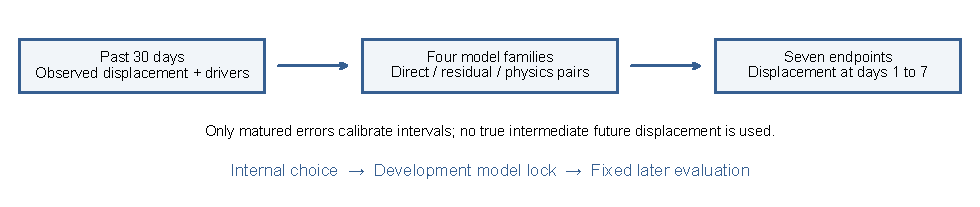
\includegraphics[width=\textwidth]{workflow.pdf}
\captionof{figure}{所有模型遵守同一观测截止。未来驱动采用当时可计算的简单场景，概率层统一使用最近 90 条成熟预测误差。}

\textbf{开发段先选身份，后期保留身份。}下表为同时满足均值与区间条件的组合；误差单位 mm，RMSE 为四点各自 RMSE 的平均。
\begin{center}\footnotesize
\begin{tabular}{clrrrr}\toprule
步长 & 锁定组合 & 开发 RMSE & 后期 RMSE & 后期 CRPS & 90\% 覆盖\\\midrule
1 & 岭回归 & 0.000918 & 0.000420 & 0.000229 & 88.48\% \\
2 & 回归＋反馈 & 0.000361 & 0.000899 & 0.000296 & 93.92\% \\
3 & 回归＋反馈 & 0.000947 & 0.002399 & 0.000820 & 93.56\% \\
4 & 回归＋反馈 & 0.001953 & 0.005143 & 0.001829 & 92.41\% \\
5 & 回归＋反馈 & 0.003510 & 0.009612 & 0.003541 & 89.97\% \\
6 & 回归＋反馈 & 0.005755 & 0.016277 & 0.006185 & 87.24\% \\
7 & 回归＋反馈 & 0.008827 & 0.025580 & 0.009978 & 85.89\% \\
\bottomrule\end{tabular}
\end{center}

\textbf{“最小误差”和“共同达标”分开判断。}在线回归＋反馈在七个步长的开发 RMSE、CRPS 均最低；1 天开发覆盖率 95.81\%，略高于事前 95\% 上限，因此共同推荐按原规则选择岭回归。均值最小组合为反馈回归的 1 天预测，后期 RMSE 为 0.000209 mm。

\small 开发目标期：2018-09-01--2019-09-11；后期：2019-09-12--2020-06-30。
每点各 h 保留全部合法起点，后期样本量依次为 293、292、291、290、289、288、287。
这些误差针对公开的已处理日序列，不能直接解释成现场传感器精度或真实失稳预警精度。

\clearpage
\pagetitle{2\quad 四类模型在同一短期任务下怎样比较}
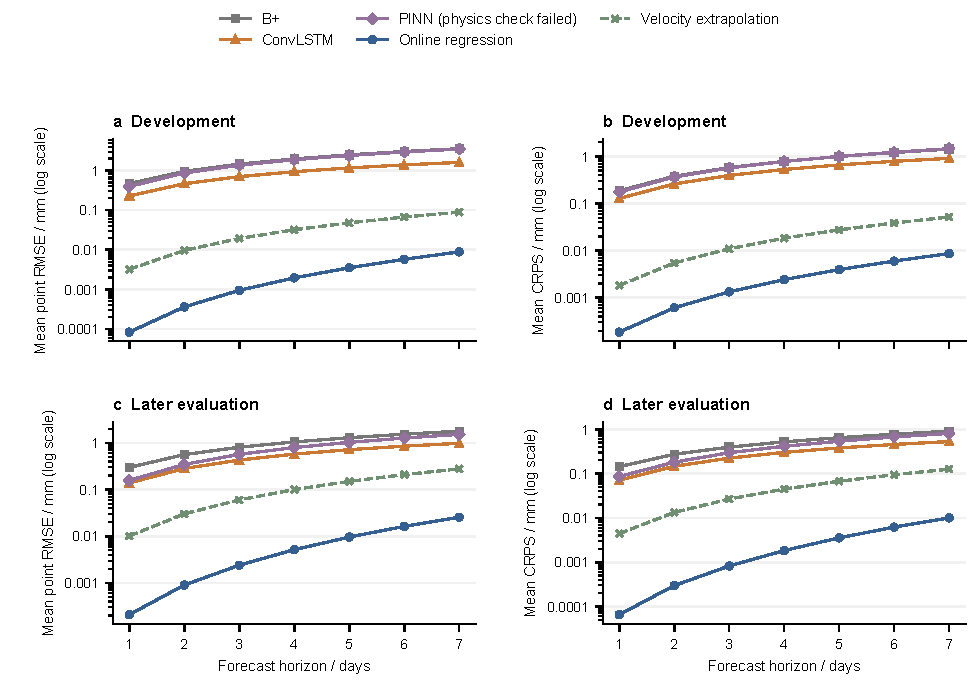
\includegraphics[width=\textwidth]{horizon_comparison.pdf}
\captionof{figure}{各家族代表按开发段同 h 的最低 RMSE 固定，再报告后期；因此代表图与第 1 页“共同推荐”的身份可能不同。纵轴为对数；点表示已发预测的整体评分，不是种子评分的平均。神经均值先作三种子等权合并。}

\textbf{固定看最长步长 7 天。}下表同时保留直接版、残差版和强对照，不按后期成绩挑选一条更好的曲线。
\begin{center}\small
\begin{tabular}{lrrr}\toprule
模型 & 开发 RMSE & 后期 RMSE & 后期 CRPS\\\midrule
锚定 B+ & 3.5570 & 1.7842 & 0.9044 \\
当天速度外推 & 0.0891 & 0.2786 & 0.1260 \\
ConvLSTM 直接版 & 1.6026 & 0.9829 & 0.5286 \\
ConvLSTM 残差版 & 2.7316 & 0.9149 & 0.5188 \\
PINN 方程约束版 & 3.4947 & 1.5275 & 0.8101 \\
岭回归直接版 & 0.0793 & 0.0373 & 0.0215 \\
岭回归残差版 & 0.0904 & 0.0376 & 0.0219 \\
在线回归＋反馈 & 0.0088 & 0.0256 & 0.0100 \\
在线回归＋反馈＋物理误差 & 0.0093 & 0.0265 & 0.0105 \\
\bottomrule\end{tabular}
\end{center}

\small ConvLSTM 两版都优于本轮 B+，但仍未超过当天速度外推。
PINN 完成训练，但其神经状态未通过独立物理重放检查，表中仍保留原神经输出；本结论限于这次固定结构。
在线回归方案还使用多尺度趋势、在线更新及误差反馈，不能把全部优势归因于“线性模型优于深度学习”。

\clearpage
\pagetitle{3\quad ATU1、ATU5：完整后期的 7 天预测}
\small 每点依次为累计位移、7 日总增量、实测减预测均值。蓝带为相对均值的 90\% 边际预测区间；误差落在蓝带内即被覆盖。累计曲线重合仍需由增量和误差图核对。
\normalsize\par\vspace{2mm}
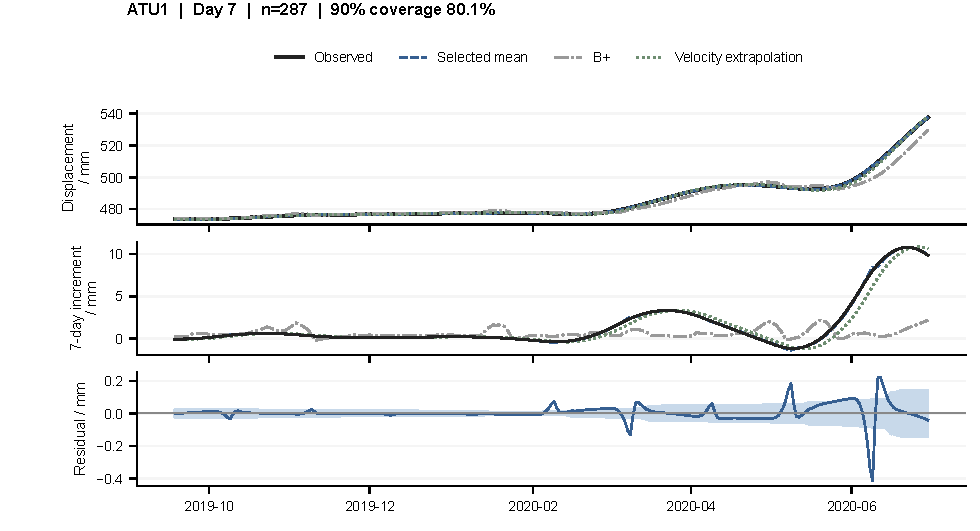
\includegraphics[width=\textwidth]{forecast_atu1_h7.pdf}
\captionof{figure}{ATU1：在线回归＋反馈，7 天后期 RMSE 0.0513 mm，90\% 区间覆盖 80.14\%。}

\vspace{4mm}
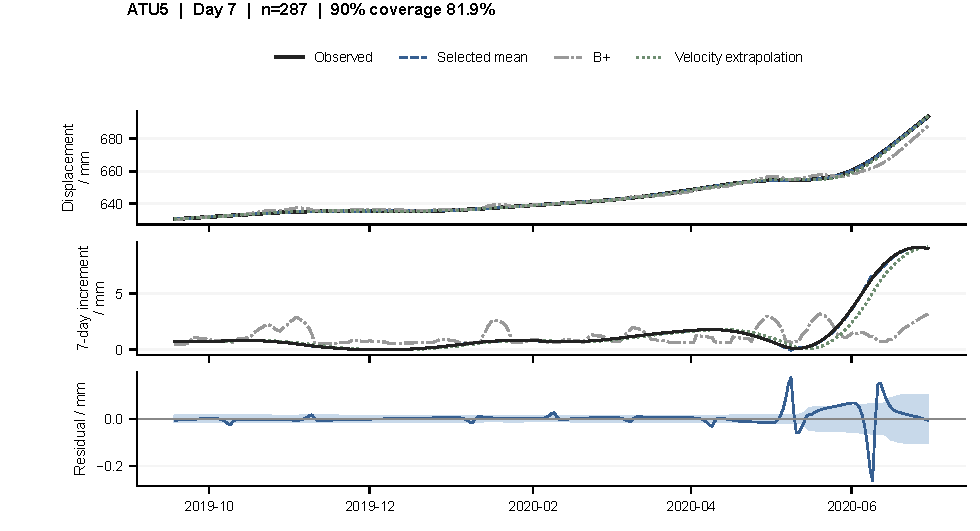
\includegraphics[width=\textwidth]{forecast_atu5_h7.pdf}
\captionof{figure}{ATU5：在线回归＋反馈，7 天后期 RMSE 0.0345 mm，90\% 区间覆盖 81.88\%。}

\small 两点覆盖率较低，ATU1 仅略高于本轮逐点 80\% 下界。困难尾段与误差尖峰全部保留，尚不能把“过工作条件”理解为已充分覆盖所有异常变化。

\clearpage
\pagetitle{4\quad MJ3、MJ1：同样保留全部后期日期}
\small 图中每条点日预测都在目标日前 7 天发出，之后未被新预测覆盖；两点均为 287 个合法起点。不同面板纵轴尺度分别标注，增量单位为 mm，未转换为单日速度。
\normalsize\par\vspace{2mm}
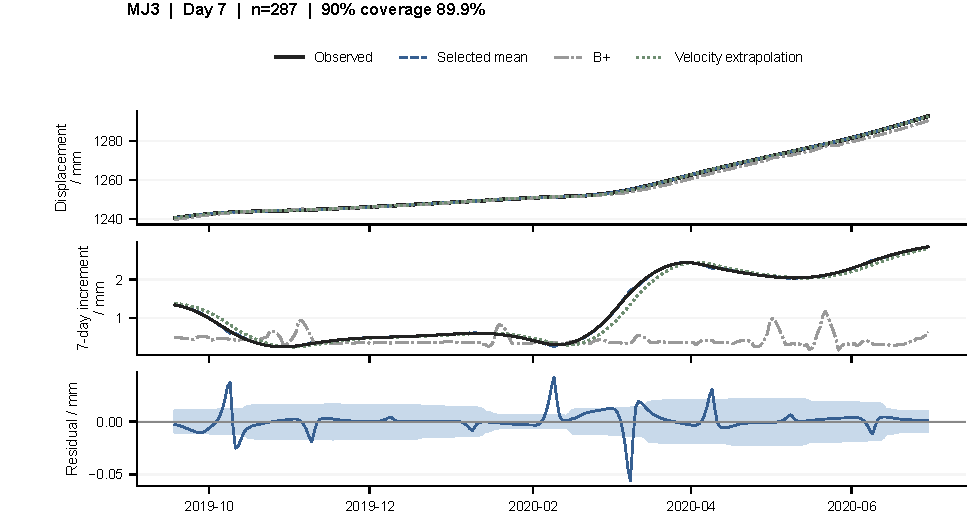
\includegraphics[width=\textwidth]{forecast_mj3_h7.pdf}
\captionof{figure}{MJ3：在线回归＋反馈，7 天后期 RMSE 0.0089 mm，90\% 区间覆盖 89.90\%。}

\vspace{4mm}
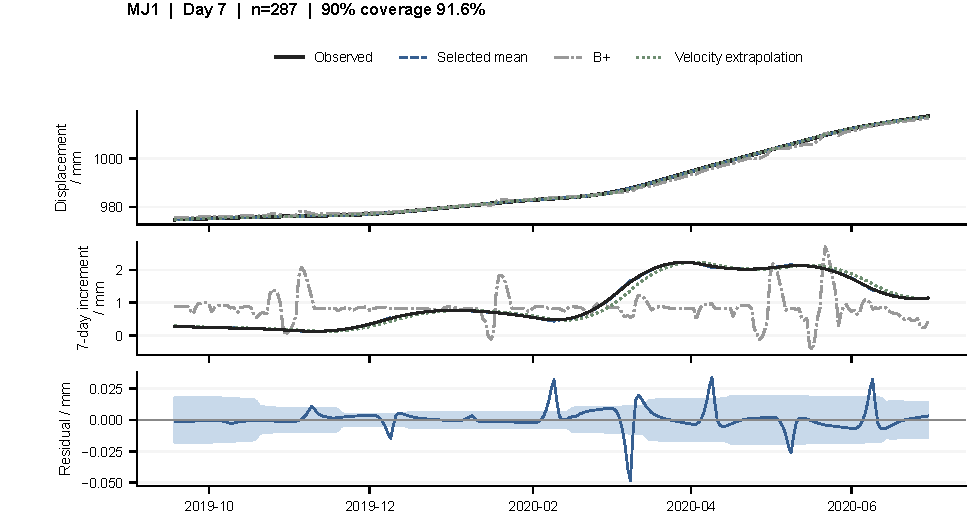
\includegraphics[width=\textwidth]{forecast_mj1_h7.pdf}
\captionof{figure}{MJ1：在线回归＋反馈，7 天后期 RMSE 0.0077 mm，90\% 区间覆盖 91.64\%。}

\small 当前最优均值属于监督回归与成熟误差反馈。B+ 在这里提供对照和可选物理误差参照；这组小误差主要来自近期位移信息，尚无稳定的额外物理增益证据。

\clearpage
\pagetitle{5\quad 残差和物理信息有没有额外收益}
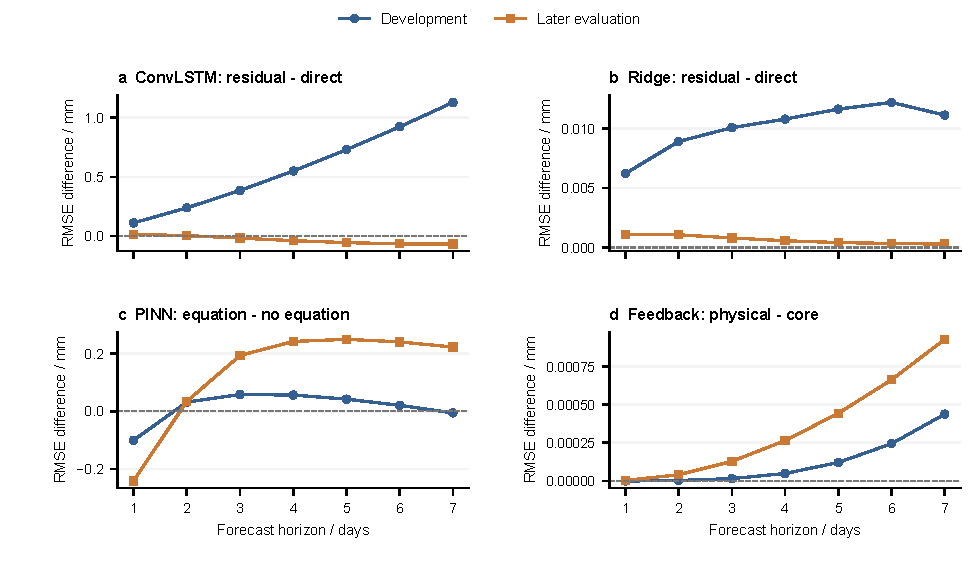
\includegraphics[width=\textwidth]{paired_effects.pdf}
\captionof{figure}{固定配对的四点平均 RMSE 差值，负值表示前一版本更好。四个面板纵轴尺度不同：残差输出、方程约束与物理误差参照是不同问题，不能混为同一种增益。}

\begin{center}\footnotesize
\begin{tabular}{lrrr}\toprule
7 天后期的概率表现 & 90\% 覆盖 & 宽度／mm & 区间评分／mm\\\midrule
锚定 B+ & 78.66\% & 4.1382 & 9.2460 \\
当天速度外推 & 75.35\% & 0.4296 & 1.3601 \\
岭回归直接版 & 86.67\% & 0.1518 & 0.2223 \\
在线回归＋反馈 & 85.89\% & 0.0415 & 0.1116 \\
在线回归＋反馈＋物理误差 & 85.80\% & 0.0420 & 0.1148 \\
\bottomrule\end{tabular}
\end{center}

\small
\textbf{这次的取舍。}ConvLSTM 残差版在开发段更差，在后期部分步长稍好；岭回归残差版未获得稳定增益。加入 B+ 一日误差后的反馈方案总体略退步。PINN 集成均值与独立 C 重放最大相差约 1.2763 mm，高于 0.01 mm 上限，停止这版结构。

\textbf{值得保留什么。}保留在线趋势回归＋短期误差反馈及共同成熟误差校准，固定 1--7 天任务和完整对照。
7 天反馈回归相对速度外推的 RMSE 差为 $-0.2530$ mm，30 日成块重采样的描述性 95\% 区间为 $[-0.3762,-0.0932]$ mm；不据此宣称新独立泛化证据。

\textbf{下一步。}先把这套短期方法写清楚，再单独确定预警对象、事件标签和阈值，评价误报、漏报与提前量；本轮没有验证真实失稳预警。
公开四条日序列具有强月内三次数值结构，原始日值当时是否可得仍未知，且评价期已被多轮探索使用。它们限制外推主张，也不自动否定本次保存的预测改善。

\vfill
{\footnotesize\color{gray}核验：36 次固定神经拟合、7800 次更新；427 项哈希、14508 个分布锁和 61152 个评分单元通过复算。完整七步长指标、配对统计、三种子结果、原始模型及 31 幅图件随版本保存。}
\end{document}
